\documentclass[]{final_report}
\usepackage{graphicx}
\usepackage{hyperref}
\usepackage[final]{pdfpages}
\usepackage{natbib}


%%%%%%%%%%%%%%%%%%%%%%
%%% Input project details
\def\studentname{James King}
\def\reportyear{2018}
\def\projecttitle{Cooperative Strategies in Multi-Agent Systems}
\def\supervisorname{Kostas Stathis}
\def\degree{BSc (Hons) in Computer Science}
\def\fullOrHalfUnit{Full Unit} % indicate if you are doing the project as a Full Unit or Half Unit
\def\finalOrInterim{Interim Report} % indicate if this document is your Final Report or Interim Report

\begin{document}

\maketitle

%%%%%%%%%%%%%%%%%%%%%%
%%% Declaration

\chapter*{Declaration}

This report has been prepared on the basis of my own work. Where other published and unpublished source materials have been used, these have been acknowledged.

\vskip3em

Word Count: 

\vskip3em

Student Name: \studentname

\vskip3em

Date of Submission: 

\vskip3em

Signature:

\newpage

%%%%%%%%%%%%%%%%%%%%%%
%%% Table of Contents
\tableofcontents\pdfbookmark[0]{Table of Contents}{toc}\newpage

%%%%%%%%%%%%%%%%%%%%%%
%%% Your Abstract here

\begin{abstract}

\end{abstract}
\newpage

\chapter{Aims, Objectives and Literary Survey}
\section{The Problem}
To understand the aims and objectives of this project we must first grasp the history of the study of interaction between biological and computational agents (often known as intelligent agents in the field of computer science). It is important to distinguish between biological and computational agents as the study of natural selection and the evolution of cooperation in biological agents (biological lifeforms such as ourselves) has a long and separate history from the study of computational agents in computer science.\\
The background I am about to explain is covered in my first two reports: on the evolution of cooperation in relation to game-theory and different game-theoretic mechanisms to aid it and on indirect reciprocity, strategies for agents and the development of a concrete model to implement. I will be applying this knowledge in a more convenient format for the interim report here, but if you are interested in a reading more in depth study by myself on this topic I suggest reading these two.\\
As explained in my first report (on the evolution of cooperation in relation to game-theory and different game-theoretic mechanisms to aid it) early darwinian evolutionary theory was groundbreaking, but both opponents and even proponents of evolution such as Peter Kropotkin~\cite{kropotkin1902mutual} a Russian evolutionary scientist and political activist found it fell short in explaining cooperative phenomena.\\
Cooperation is the idea of helping others at a detriment or cost to yourself. Of course this is a key part of the natural world, like the act of parents supporting their children and vice-versa in human family groups. There are even interspecies examples such as that of the Meerkat and Drongo Bird~\cite{bbcafrica}.\\
The problematic question posed by this phenomena is that natural selections idea: the survival of the fittest~\cite{spencer1864principles}, pushes individuals to compete for resources, so why does cooperation exist when there is a process actively pushing for competition? How did cooperation evolve in a world focused on competition?

\section{Cooperation Aids}
There have been a number of attempts to explain the phenomena of cooperation~\cite{kropotkin1902mutual, selfish_gene, evolution_of_cooperation, five_rules_coop}. Richard Dawkins in his book the selfish gene~\cite{selfish_gene} attempted to explain how the idea that we do not act towards improving our personal fitness, but that the real replicator in natural selection is the gene not the individual and as such the gene is selfish and wishes to propagate itself.\\
This idea comes under the banner of kinship theories, highlighted by Axelrod and Hamilton in their paper the evolution of cooperation~\cite{evolution_of_cooperation} as one of the theories seeking to explain cooperation. Hamilton wrote a paper on kinship theory earlier on~\cite{kinhamilton} explaining his version of kinship theory in which agents are encouraged to cooperate as they work on improving `inclusive fitness over 

\section{Theory Surrounding Intelligent Agents and Multi-Agent Systems}

\section{Relevance of The Problem to Multi-Agent Systems}

\section{Aims and Objectives}

\chapter{Planning and Timescale}
Provide timeline of completed work and an updated one for next term.

\chapter{Summary of Completed Work}
Relevance to project aims
\begin{itemize}
	\item Evolution of cooperation report
	\item Indirect reciprocity report
	\item System design report
	\item A prolog web app for proof of concept
	\item A flask web application to begin educational tool and as a proof of concept
	\item API documentation
	\item Agents service:
	\begin{itemize}
		\item Vertical slice of 3 strategies: perceive, revise, decide
		\item Use of mvfcec for revise
		\item Agent management
		\item Test agents revision
		\item Get strategies implementation
		\item 
	\end{itemize}
\end{itemize}
Agents service, flask web app, environment, two reports

\section{Practical}

\subsection{Proof Of Concepts}

\subsection{System Design}

\subsection{Agents Service and API}
RESTful API. MVFCEC. Agent Template.

\subsection{The Environment}

\subsection{Tools, Techniques and Processes}

TDD, UML, Processes in VCS, Testing Strategy

\section{Theory}
Summary of the reports and theory work.
\subsection{Evolution of Cooperation Report}

\subsection{Indirect Reciprocity Report}

\subsection{System Design Report}

%%%% ADD YOUR BIBLIOGRAPHY HERE
\newpage
\bibliography{../../refs.bib}{}
\bibliographystyle{plain}
\addcontentsline{toc}{chapter}{Bibliography}
\footnote{A lot of my background theory work has been completed in my earlier reports so many of the references appear in those reports (see appendix)}
\label{endpage}

\chapter{Diary}

\chapter{Appendix}
Introduce the two reports

%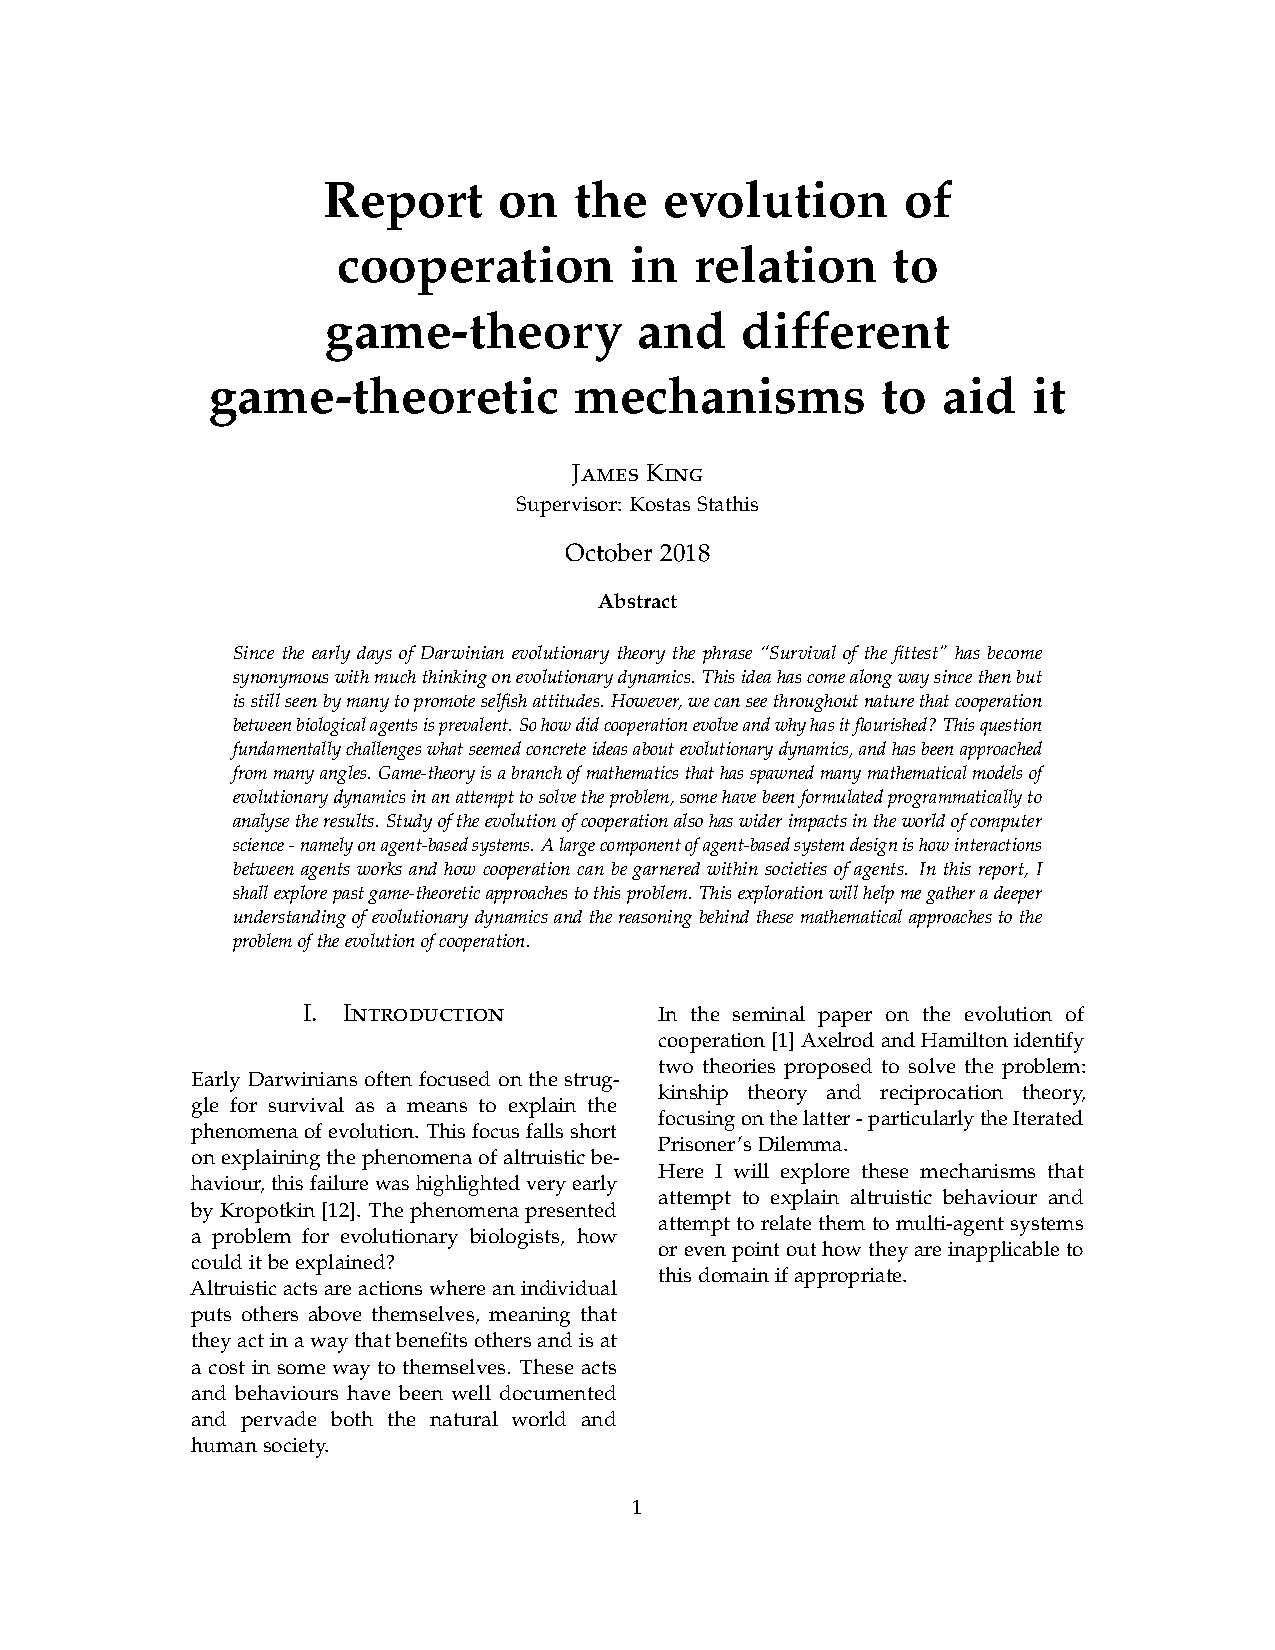
\includepdf[pages=-]{../../EvolCoop/EvolCoopReport.pdf}

%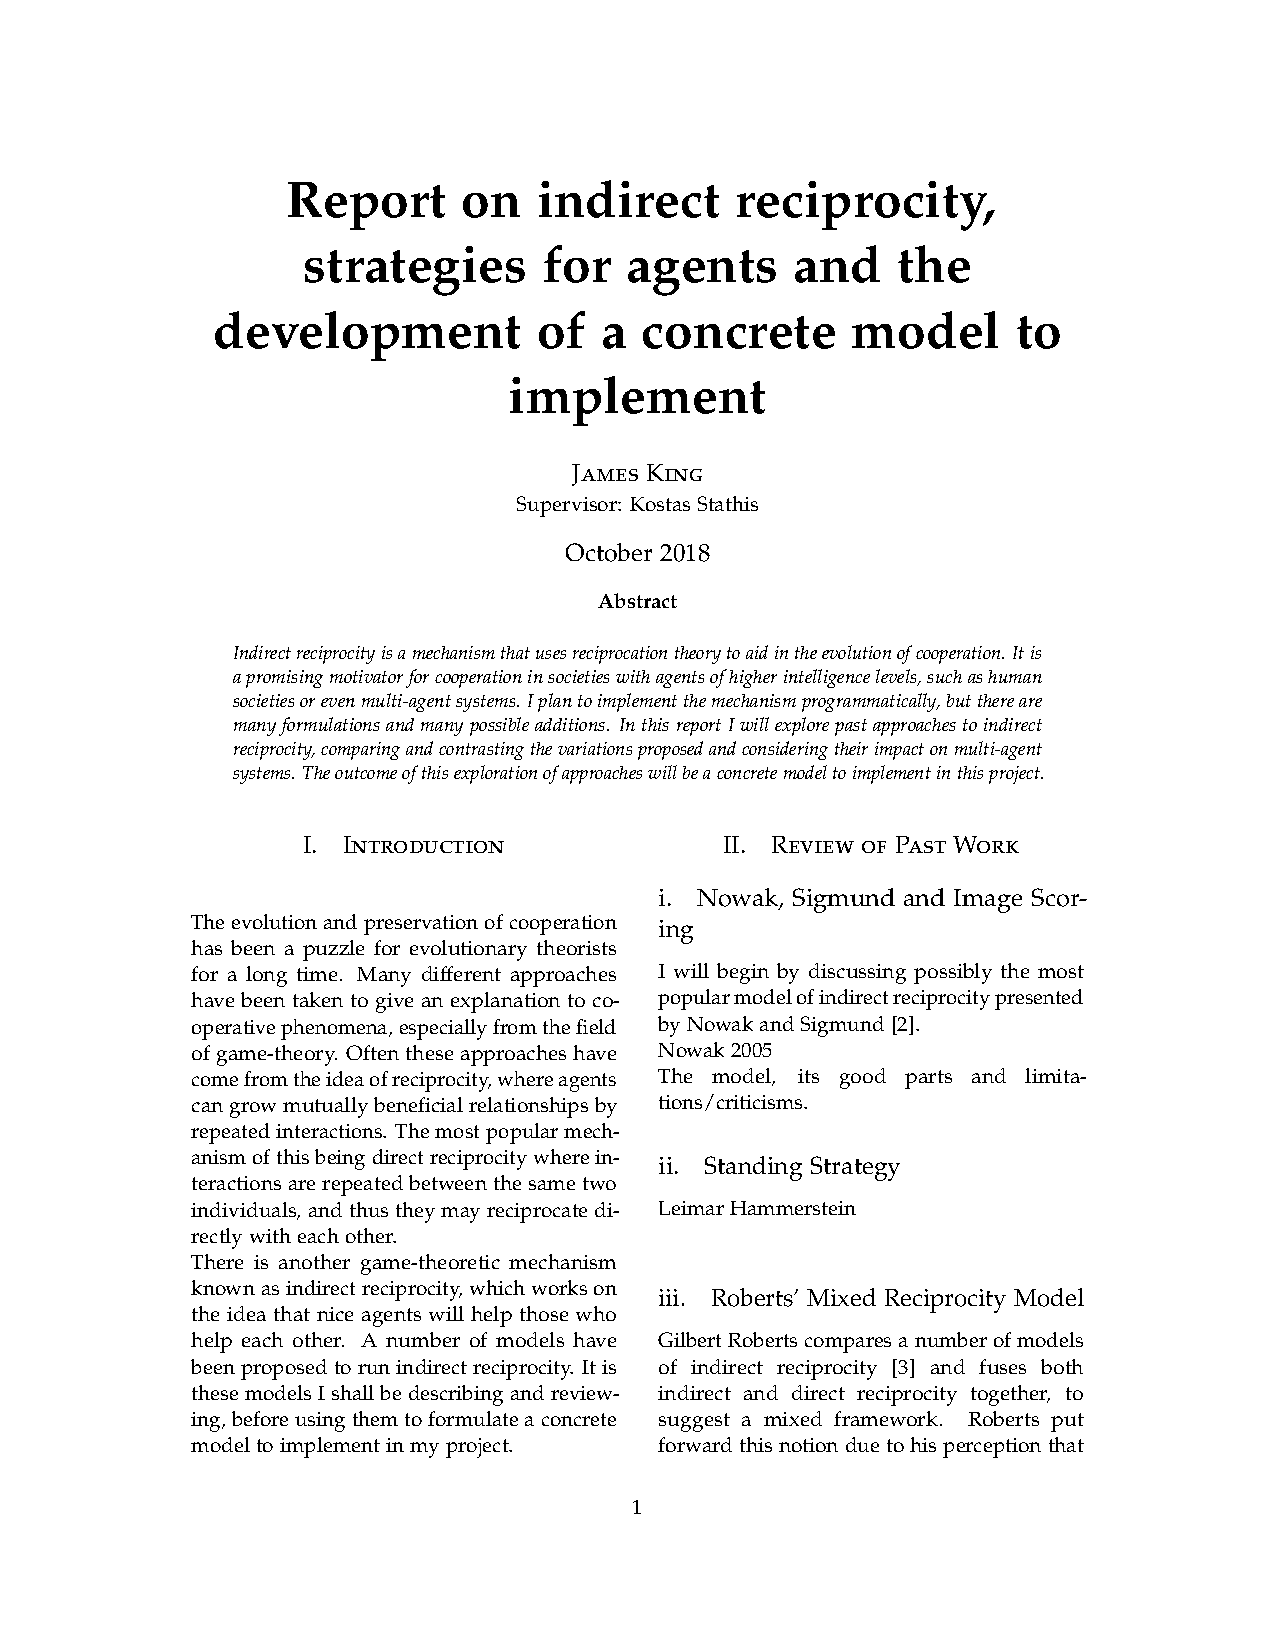
\includepdf[pages=-]{../../IndirRec/IndirRec.pdf}

\end{document}

\end{article}
